\Aufgabe[Simulation as refinement \hfill\textbf{(2 Points)}]
 
Given a \texttt{C} program and a set $AP$ of atomic propositions,
one can construct a Kripke structure over $AP$ which models the behaviour of the program with respect to the atomic propositions. 
For example, given the following program:

\begin{verbatim}
int x = 0, y = 0;
l0:
    for (int i = 0; i < 2; i++)
l1:     x = 1;
    y = *;
    if (y != 0)
l2:     x = 1;
    else
l3:     x = 0;
    goto l0;
\end{verbatim}

One may construct the following Kripke structure over $AP=\{x=0, y=0\}$
as follows:

\begin{center}
	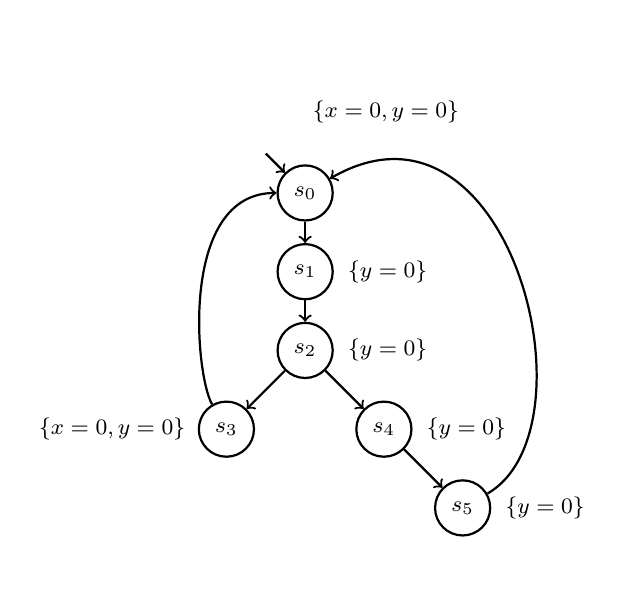
\begin{tikzpicture}[->,scale=1,label distance=0mm]
		\tikzstyle{every node}=[draw,shape=circle,minimum size=7mm,font=\footnotesize];
    \tikzstyle{every path}=[draw,thick];
    \node at (0, 0)   (s0) [label=above right:${ \{x=0,y=0\} }$]  {$s_0$};
    \node at (0, -1)  (s1) [label=right:${ \{y=0\} }$] {$s_1$};
    \node at (0, -2)  (s2) [label=right:${ \{y=0\} }$] {$s_2$};
    \node at (-1, -3) (s3) [label=left:${ \{x=0,y=0\} }$] {$s_3$};
    \node at (1, -3)  (s4) [label=right:${ \{y=0\} }$] {$s_4$};
    \node at (2, -4)  (s5) [label=right:${ \{y=0\} }$] {$s_5$};

    \draw (-0.5, 0.5) to (s0);
    \draw (s0) to (s1);
    \draw (s1) to (s2);
    \draw (s2) to (s3);
    \draw (s2) to (s4);
    \draw (s3) .. controls +(120:8mm) and +(left:16mm) .. (s0);
    \draw (s4) to (s5);
    \draw (s5) .. controls +(30:20mm) and +(30:30mm) .. (s0);
	\end{tikzpicture}
\end{center}
In the example above, the special
form of assignment \texttt{y = *} denotes a non-deterministic assignment
to~\texttt{y} of any value from the domain of \texttt{y}, e.g., it can be
assigned concurrently by another thread.
The effect of a statement sequence residing under the same label $\ell_j$ may
be merged into one state, whereas the effect of statements marked with
distinct labels $\ell_j$ and $\ell_k$, $j \ne k$, must not be merged into one
state.

\paragraph{a)}
Construct a Kripke structure $K$ over
$AP=\{port\_o=0,port\_o=1,port\_o=2,port\_o=3\}$ for the following program:

\begin{verbatim}
int locked_dev = 0, port_o = 0, port_i = 0;
l0:
    for (int i = 0; i < 3; i++)
l1:     port_o = 1;

    port_i = *;
    if (port_i < 3) {
        goto l0;
    }
    do {
l2:     port_o = 2; locked_dev = *;
    } while (locked_dev);
l3: locked_dev = 1; port_i = *;
    if (port_i == 1)
l4:     port_o = 1;
    else
l5:     port_o = 3;
l6: port_o = 0; locked_dev = 0;
    goto l0;
\end{verbatim}


\paragraph{b)}
Give simulation relations between $K$ and the following Kripke structures
 $S'$ (left) and $S''$ (right):

\begin{center}
	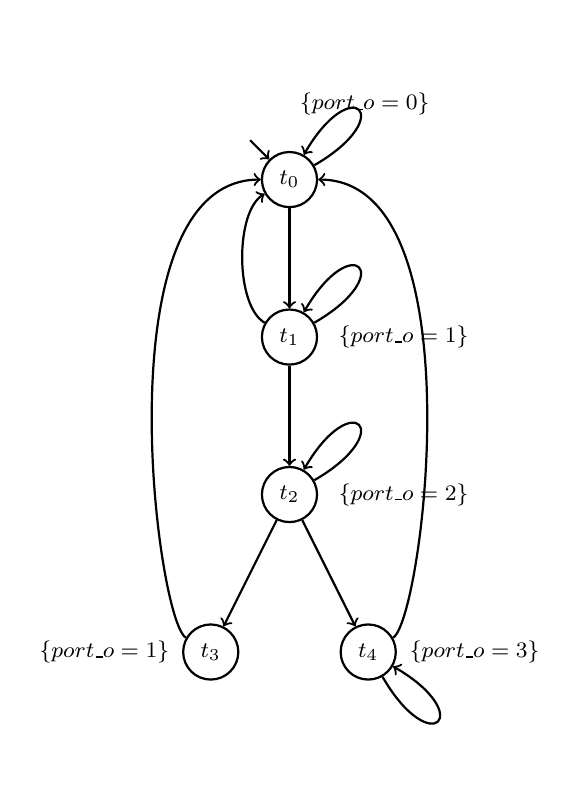
\begin{tikzpicture}[->,scale=1,label distance=0mm]
		\tikzstyle{every node}=[draw,shape=circle,minimum size=7mm,font=\footnotesize];
    \tikzstyle{every path}=[draw,thick];
    \node at (0, 0)   (s0) [label=above right:${ \{port\_o=0\} }$]  {$t_0$};
    \node at (0, -2)  (s1) [label=right:${ \ \{port\_o=1\} }$] {$t_1$};
    \node at (0, -4)  (s2) [label=right:${ \ \{port\_o=2\} }$] {$t_2$};
    \node at (-1, -6) (s3) [label=left:${ \{port\_o=1\} }$] {$t_3$};
    \node at (1, -6)  (s4) [label=right:${ \{port\_o=3\} }$] {$t_4$};

    \draw (-0.5, 0.5) to (s0);
    \draw (s0) to (s1);
    \draw (s0)  .. controls +(30:16mm) and +(60:16mm) .. (s0);
    \draw (s1)  .. controls +(150:8mm) and +(210:8mm) .. (s0);
    \draw (s1)  .. controls +(30:16mm) and +(60:16mm) .. (s1);
    \draw (s1) to (s2);
    \draw (s2)  .. controls +(30:16mm) and +(60:16mm) .. (s2);
    \draw (s2) to (s3);
    \draw (s2) to (s4);
    \draw (s3) .. controls +(150:8mm) and +(left:24mm) .. (s0);
    \draw (s4) .. controls +(30:8mm) and +(right:24mm) .. (s0);
    \draw (s4)  .. controls +(300:16mm) and +(330:16mm) .. (s4);
    	\end{tikzpicture}
	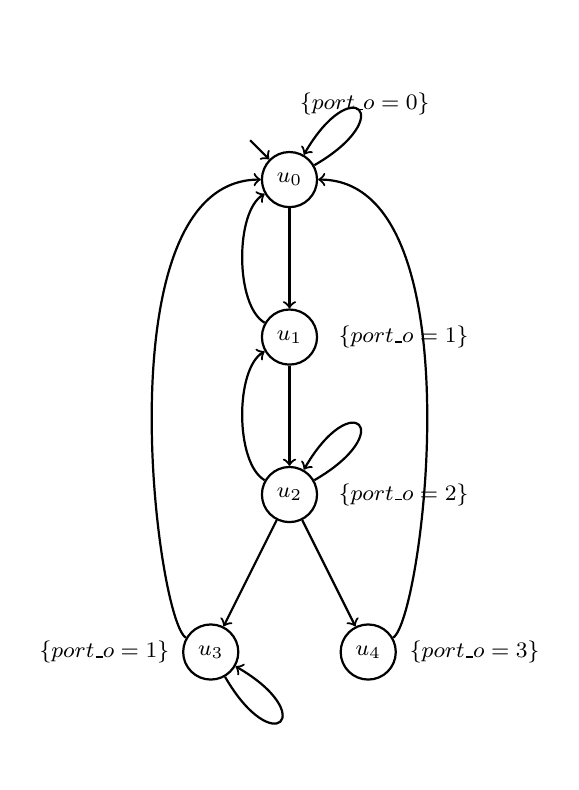
\begin{tikzpicture}[->,scale=1,label distance=0mm]
		\tikzstyle{every node}=[draw,shape=circle,minimum size=7mm,font=\footnotesize];
    \tikzstyle{every path}=[draw,thick];
    \node at (0, 0)   (s0) [label=above right:${ \{port\_o=0\} }$]  {$u_0$};
    \node at (0, -2)  (s1) [label=right:${ \ \{port\_o=1\} }$] {$u_1$};
    \node at (0, -4)  (s2) [label=right:${ \ \{port\_o=2\} }$] {$u_2$};
    \node at (-1, -6) (s3) [label=left:${ \{port\_o=1\} }$] {$u_3$};
    \node at (1, -6)  (s4) [label=right:${ \{port\_o=3\} }$] {$u_4$};

    \draw (-0.5, 0.5) to (s0);
    \draw (s0) to (s1);
    \draw (s0)  .. controls +(30:16mm) and +(60:16mm) .. (s0);
    \draw (s1)  .. controls +(150:8mm) and +(210:8mm) .. (s0);
    \draw (s2)  .. controls +(150:8mm) and +(210:8mm) .. (s1);
    \draw (s1) to (s2);
    \draw (s2)  .. controls +(30:16mm) and +(60:16mm) .. (s2);
    \draw (s2) to (s3);
    \draw (s2) to (s4);
    \draw (s3) .. controls +(150:8mm) and +(left:24mm) .. (s0);
    \draw (s3) .. controls +(300:16mm) and +(330:16mm) .. (s3);
    \draw (s4) .. controls +(30:8mm) and +(right:24mm) .. (s0);
    	\end{tikzpicture}
\end{center}

\textbf{Solution:}\\

\begin{enumerate}
\item Kripke structure $K$:

\begin{center}
\begin{tikzpicture}[->,scale=1,label distance=0mm]
	\tikzstyle{every node}=[draw,shape=circle,minimum size=7mm,font=\footnotesize];
    \tikzstyle{every path}=[draw,thick];

    \node at (0, 0)   (s0) [label=left:${ \{port\_o=0\} }$]  {$s_0$};
    \node at (0, -1.5)  (s1) [label=right:${ \ \{port\_o=1\} }$] {$s_1$};
    \node at (0, -3)  (s2) [label=right:${ \ \{port\_o=1\} }$] {$s_2$};
    \node at (0, -4.5)  (s3) [label=right:${ \ \{port\_o=1\} }$] {$s_3$};
    \node at (-1.5, -6) (s4) [label=left:${ \{port\_o=1\} }$] {$s_4$};
    \node at (1.5, -6)  (s5) [label=right:${ \{port\_o=2\} }$] {$s_5$};
    \node at (0, -7.5) (s6) [label=left:${ \{port\_o=1\} }$] {$s_6$};
    \node at (3, -7.5)  (s7) [label=right:${ \{port\_o=3\} }$] {$s_7$};
    \node at (1.5, -9)  (s8) [label=left:${ \ \{port\_o=0\} }$] {$s_8$};

    \draw (-0.5, 0.5) to (s0);
    \draw (s0) to (s1);
    \draw (s1) to (s2);
    \draw (s2) to (s3);
    \draw (s3) to (s4);
    \draw (s3) to (s5);
    \draw (s4) .. controls +(120:15mm) and +(left:20mm) .. (s1);
    \draw (s5) .. controls +(30:16mm) and +(60:16mm) .. (s5);
    \draw (s5) to (s6);
    \draw (s5) to (s7);
    \draw (s6) to (s8);
    \draw (s7) to (s8);
    \draw (s8)  .. controls +(0:96mm) and +(25:25mm) .. (s0);
\end{tikzpicture}
\end{center}

\item $S'$ simulates $K$ with the following simulation relation:
$$H' = \{(s_0,t_0),(s_1,t_1),(s_2,t_1),(s_3,t_1),(s_4,t_1),(s_5,t_2),(s_6,t_3),(s_7,t_4),(s_8,t_0)\},$$
and $S''$ simulates $K$ with the following simulation relation,
$$H'' = \{(s_0,u_0),(s_1,u_3),(s_2,u_3),(s_3,u_1),(s_4,u_3),(s_5,u_2),(s_6,u_1),(s_6,u_3),(s_7,u_4),(s_8,u_0)\}.$$
%$K$ doesn't simulate neither $S'$ nor $S''$, because there doesn't exist any state with AP $\{port\_o=0\}$ which has a path to $\{port\_o=0\}$ and $\{port\_o=1\}$...
\end{enumerate}
